% ============================================================
% Lecture 3 -- Data Visualization using ggplot()-geoms
% ============================================================
\section{Data Visualization using ggplot()-geoms}\label{sec:L03}

\lectureheader{3}{EP8uu2k5WfA}{Week-1 slides \texttt{Jan26notes.pdf}, part ``ggplot()-geoms'' to ``layered grammar of graphics''; recap slides at the start of \texttt{Feb2.pdf}}

\begin{guiding*}
By the end of this lecture you should be able to:
\begin{itemize}
  \item explain what a \emph{geom} is and switch between \texttt{geom\_point} and \texttt{geom\_smooth};
  \item give mappings globally or per layer, and use a different data subset for one layer;
  \item explain the \emph{statistical transformation} behind a bar chart (\texttt{stat\_count}) and use \texttt{stat\_summary};
  \item use position adjustments (\texttt{dodge}) and coordinate systems (\texttt{coord\_flip}, \texttt{coord\_polar});
  \item write down the full layered grammar-of-graphics template.
\end{itemize}
\end{guiding*}

\subsection{Recap}
In \cref{sec:L02} we built scatter plots with \texttt{ggplot(data) + geom\_point(aes(...))},
added a third variable through an aesthetic, and split plots into facets. This lecture
completes the grammar. We still use the \texttt{mpg} data.

\subsection{Geoms}
\begin{definition}[Geom]\label{def:L03-geom}
A \vocab{geom} is the geometrical object that a plot uses to represent data: points, lines,
bars, boxes, and so on.
\end{definition}
The same data can be drawn with different geoms.
\begin{itemize}
  \item \texttt{ggplot(mpg) + geom\_point(aes(x = displ, y = hwy))} draws the scatter plot.
  \item \texttt{ggplot(mpg) + geom\_smooth(aes(x = displ, y = hwy))} draws a \emph{smooth curve} fitted to the same points, with a grey confidence band.
\end{itemize}
The smooth curve decreases from about $29$ mpg at $2$ litres to about $17$--$18$ mpg at
$5$ litres. The default R smoother (local \emph{quadratic} fits) then turns up slightly for the
largest engines. The upturn is caused by the 2-seaters we saw in \cref{ex:L02-colour}. The
local-\emph{linear} LOWESS used in the Python notebook flattens out instead, and it gives
about $15.5$ mpg at $6$ litres.

\begin{note}[Supplementary: what \texttt{geom\_smooth} fits]
For fewer than $1000$ observations the default smoother is \vocab{LOESS} (locally estimated
scatterplot smoothing). At each point $x_0$ it fits a low-degree polynomial to the nearby data
by \emph{weighted least squares}. Points closer to $x_0$ get larger weights. The value of that
local fit at $x_0$ is the curve's height. So even the ``model-free'' smooth curve is built from
many small least-squares fits: the subject of this course, applied locally. With
\texttt{method = "lm"} one gets the single global least-squares line instead. The instructor
uses this option in Week~5 (\cref{sec:L15}).
\end{note}

\subsection{Global and local mappings}
Mappings can be given once, in \texttt{ggplot()}, and are then inherited by every layer:
\codeline{ggplot(mpg, aes(x = displ, y = hwy)) + geom\_point(aes(color = drv)) + geom\_smooth() + scale\_colour\_viridis\_d()}
Here $x$ and $y$ are \emph{global}, while \texttt{color = drv} is \emph{local} to the point
layer. The points are coloured by drive type (4, f, r), and a single smooth curve is fitted to
all the data.

A layer can even use different data. The instructor's second version replaces the smooth by
\codeline{geom\_smooth(data = filter(mpg, drv == "4"))}
Here \texttt{filter} keeps only the four-wheel-drive cars, so the smooth curve describes only
those cars while the points still show every car.

\subsection{Bar charts and statistical transformations}
\begin{example}[Counts by class]\label{ex:L03-count}
\texttt{ggplot(mpg) + stat\_count(aes(x = class))} and
\texttt{ggplot(mpg) + geom\_bar(aes(x = class))} produce the \emph{same} bar chart. The counts
agree with \texttt{table(mpg\$class)}:
\begin{center}
\begin{tabular}{ccccccc}\hline
2seater & compact & midsize & minivan & pickup & subcompact & suv\\\hline
5 & 47 & 41 & 11 & 33 & 35 & 62\\\hline
\end{tabular}
\end{center}
The seven counts add up to $234$, the number of rows.
\end{example}

\begin{definition}[Stat]\label{def:L03-stat}
A \vocab{stat} is a \emph{statistical transformation} applied to the data before display. For a
bar chart the stat is \texttt{count}: for each level $c$ of the $x$-variable it computes
$n_c=\#\{i: x_i=c\}$ and passes the pairs $(c,n_c)$ to the bar geom. Every geom has a default
stat, and every stat has a default geom. \texttt{geom\_bar} uses \texttt{stat\_count}, and
\texttt{stat\_count} uses \texttt{geom\_bar}. This is why the two commands above are
interchangeable. \texttt{ggplot2} provides over $20$ stats (see \texttt{?stat\_bin}).
\end{definition}

\begin{example}[\texttt{stat\_summary}]\label{ex:L03-summary}
\codeline{ggplot(mpg) + stat\_summary(aes(x = class, y = hwy), fun.min = min, fun.max = max, fun = median)}
For each class this draws a point at the median highway mileage and a vertical line from the
minimum to the maximum. The values plotted are:
\begin{center}
\begin{tabular}{lccccccc}\hline
 & 2seater & compact & midsize & minivan & pickup & subcompact & suv\\\hline
min & 23 & 23 & 23 & 17 & 12 & 20 & 12\\
median & 25 & 27 & 27 & 23 & 17 & 26 & 17.5\\
max & 26 & 44 & 32 & 24 & 22 & 44 & 27\\\hline
\end{tabular}
\end{center}
Pickups and SUVs have the lowest median mileage. Compacts and subcompacts have the largest
spread: their maxima of $44$ belong to a few very efficient cars.
\end{example}

\subsection{Position adjustments and coordinate systems}
\begin{itemize}
  \item \texttt{geom\_bar(aes(x = class, fill = trans))} \emph{stacks} the bars, splitting each class bar by transmission type. The \texttt{fill} aesthetic colours the inside of the bars.
  \item \texttt{position = "dodge"} puts the pieces \emph{side by side}. This makes the counts within a class easier to compare.
  \item \texttt{coord\_flip()} swaps the axes, giving horizontal bars. This is handy for long category names.
  \item \texttt{coord\_polar()} uses polar coordinates. The bar chart becomes a ``Coxcomb'' chart.
\end{itemize}

\begin{figure}[ht]
\centering
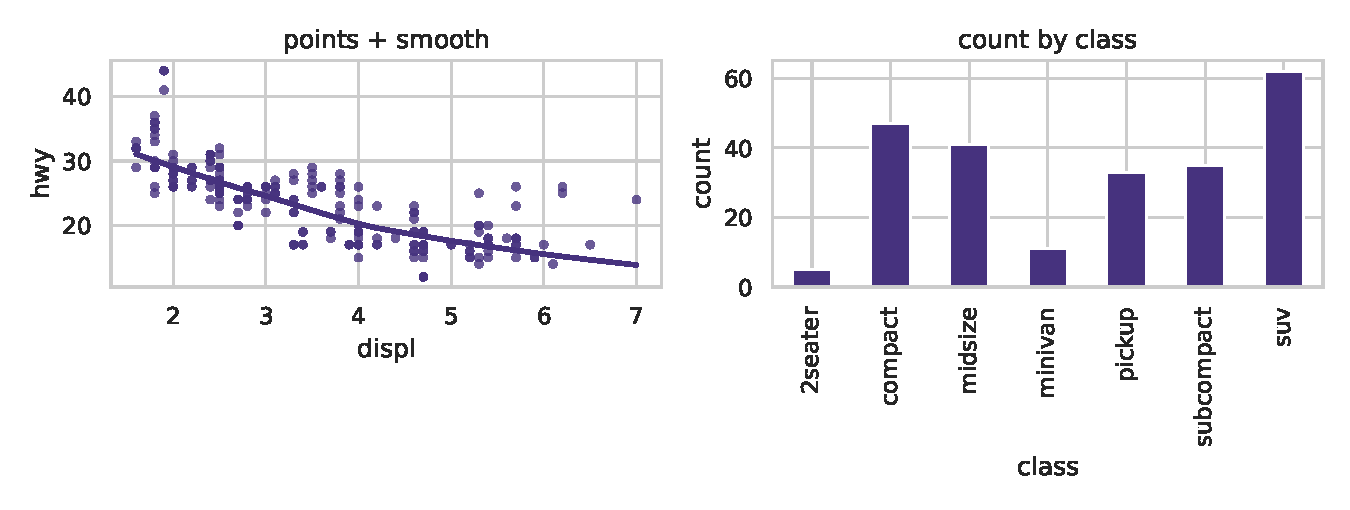
\includegraphics[width=0.95\textwidth]{figures/L03_geoms.pdf}
\caption{Left: points with a LOESS smooth. Right: the count stat behind a bar chart.}
\label{fig:L03-geoms}
\end{figure}

\subsection{The layered grammar of graphics}
\begin{definition}[Layered grammar of graphics]\label{def:L03-grammar}
Every \texttt{ggplot2} graph fits the template
\begin{center}
\begin{minipage}{0.6\textwidth}
\ttfamily
ggplot(data = <DATA>) +\\
\quad <GEOM\_FUNCTION>(\\
\quad\quad mapping = aes(<MAPPINGS>),\\
\quad\quad stat = <STAT>,\\
\quad\quad position = <POSITION>\\
\quad ) +\\
\quad <COORDINATE\_FUNCTION> +\\
\quad <FACET\_FUNCTION>
\end{minipage}
\end{center}
The seven parameters (data, geom, mapping, stat, position, coordinates, facets) are enough to
describe almost any plot.
\end{definition}
The instructor's summary annotation lists what the week covered: scatter plots, viridis colours,
bar charts, facets, geoms and coordinate systems. The recap at the start of Week~2 calls
the grammar the ``key tool in data visualisation''.

\subsection{Computation}
\begin{center}
\small\begin{tabular}{@{}>{\raggedright\arraybackslash}p{7.3cm}>{\raggedright\arraybackslash}p{8.3cm}@{}}\hline
R & Python\\\hline
\texttt{geom\_smooth()} (LOESS) & \texttt{sns.regplot(..., lowess=True)} or \texttt{statsmodels.nonparametric.lowess}\\
\texttt{filter(mpg, drv=="4")} & \texttt{mpg[mpg.drv == "4"]}\\
\texttt{geom\_bar(aes(class))} & \texttt{sns.countplot(data=mpg, x="class")}\\
\texttt{stat\_summary(fun=median, ...)} & \texttt{mpg.groupby("class").hwy} \texttt{.agg(["min", "median", "max"])}\\
\texttt{fill=trans, position="dodge"} & \texttt{sns.countplot(..., hue="trans")}\\
\texttt{coord\_flip()} & \texttt{sns.countplot(..., y="class")}\\
\texttt{coord\_polar()} & \texttt{plt.subplot(projection="polar")} with \texttt{ax.bar}\\\hline
\end{tabular}
\end{center}
See \nb{week01/L03\_ggplot\_geoms.ipynb}.

\subsection{Summary}
\begin{itemize}
  \item A geom is the object that represents data. A stat is the transformation applied first.
  \item Mappings in \texttt{ggplot()} are global; mappings in a geom are local. Each layer may use its own data.
  \item \texttt{geom\_bar} $=$ \texttt{stat\_count} $+$ bars. \texttt{stat\_summary} draws min/median/max summaries.
  \item \texttt{position="dodge"}, \texttt{coord\_flip()} and \texttt{coord\_polar()} change the layout.
  \item The template has seven parameters: data, geom, mapping, stat, position, coordinates, facets.
\end{itemize}

\subsection{Exercises}
\begin{problem}\label{prob:L03-1}
Which stat does \texttt{geom\_histogram} use, and what does it compute? How is it related to \texttt{stat\_count}?
\end{problem}
\begin{problem}\label{prob:L03-2}
Reproduce the \texttt{stat\_summary} table of \cref{ex:L03-summary} for \texttt{cty} instead of \texttt{hwy}. Which class has the largest range?
\end{problem}
\begin{problem}\label{prob:L03-3}
Explain why \texttt{geom\_smooth(method = "lm")} gives a straight line while the default gives a curve. What quantity does the \texttt{lm} line minimise?
\end{problem}
\begin{problem}\label{prob:L03-4}
Make a dodged bar chart of \texttt{drv} within each \texttt{class} in Python. Which class contains all three drive types?
\end{problem}

\subsection{Further reading}
Wickham \& Grolemund, \emph{R for Data Science}, Chapter~3 (Sections on geometric objects,
statistical transformations, position adjustments, coordinate systems and the layered grammar).
